\documentclass[12pt,spanish,fleqn,openany,letterpaper,pagesize]{scrbook}

\usepackage[ansinew]{inputenc}
\usepackage[spanish]{babel}
\usepackage[T1]{fontenc}
\usepackage{fancyhdr}
\usepackage{epsfig}
\usepackage{epic}
\usepackage{eepic}
\usepackage{amsmath}
\usepackage{threeparttable}
\usepackage{amscd}
\usepackage{here}
\usepackage{graphicx}
\usepackage{lscape}
\usepackage{tabularx}
\usepackage{subfigure}
\usepackage{longtable}
\usepackage{cite}
\usepackage{url}
\usepackage{hyperref}
\usepackage{mathptmx}
\usepackage{helvet}
\usepackage{enumerate}
\usepackage{multirow}
\usepackage{amsmath}
\usepackage{amsfonts}
\usepackage{amssymb}
\usepackage{textcomp}
\usepackage{xcolor,colortbl}
%\usepackage{apalike}
\hyphenation{e-la-bo-ra-ron}
\hyphenation{ins-truc-ci�n}
\hyphenation{a-xio-mas}
\hyphenation{pro-ba-bi-l�s-ti-co}
\hyphenation{cu-rri-cu-lar}
\hyphenation{cir-cuns-tan-cias}
\hyphenation{de-sa-rro-llar}
\hyphenation{re-fe-ren-cia}
\hyphenation{cua-li-dad}
\hyphenation{cu-rr�-cu-lo}
\hyphenation{o-cu-rren-cia}
\hyphenation{pro-ba-bi-li-dad}
\hyphenation{de-sa-rro-llo}
\hyphenation{in-he-ren-tes}
\hyphenation{co-rres-pon-dien-tes}

\usepackage{rotating} %Para rotar texto, objetos y tablas seite. No se ve en DVI solo en PS. Seite 328 Hundebuch
                        %se usa junto con \rotate, \sidewidestable ....


\renewcommand{\theequation}{\thechapter-\arabic{equation}}
\renewcommand{\thefigure}{\textbf{\thechapter-\arabic{figure}}}
\renewcommand{\thetable}{\textbf{\thechapter-\arabic{table}}}


\pagestyle{fancyplain}%\addtolength{\headwidth}{\marginparwidth}
\textheight22.5cm \topmargin0cm \textwidth16.5cm
\oddsidemargin0.5cm \evensidemargin-0.5cm%
\renewcommand{\chaptermark}[1]{\markboth{\thechapter\; #1}{}}
\renewcommand{\sectionmark}[1]{\markright{\thesection\; #1}}
\lhead[\fancyplain{}{\thepage}]{\fancyplain{}{\rightmark}}
\rhead[\fancyplain{}{\leftmark}]{\fancyplain{}{\thepage}}
\fancyfoot{}
\thispagestyle{fancy}%


\addtolength{\headwidth}{0cm}
\unitlength1mm %Define la unidad LE para Figuras
\mathindent0cm %Define la distancia de las formulas al texto,  fleqn las descentra
\marginparwidth0cm
\parindent0cm %Define la distancia de la primera linea de un parrafo a la margen

%Para tablas,  redefine el backschlash en tablas donde se define la posici\'{o}n del texto en las
%casillas (con \centering \raggedright o \raggedleft)
\newcommand{\PreserveBackslash}[1]{\let\temp=\\#1\let\\=\temp}
\let\PBS=\PreserveBackslash

%Espacio entre lineas
\renewcommand{\baselinestretch}{1.1}

%Neuer Befehl f\"{u}r die Tabelle Eigenschaften der Aktivkohlen
\newcommand{\arr}[1]{\raisebox{1.5ex}[0cm][0cm]{#1}}

%Neue Kommandos
\usepackage{Befehle}


%Trennungsliste
\hyphenation {Reaktor-ab-me-ssun-gen Gas-zu-sa-mmen-set-zung
Raum-gesch-win-dig-keit Durch-fluss Stick-stoff-gemisch
Ad-sorp-tions-tem-pe-ra-tur Klein-schmidt
Kohlen-stoff-Mole-kular-siebe Py-rolysat-aus-beu-te
Trans-port-vor-gan-ge}

%\includeonly{Kap1/Kap1,Kap2/Kap2}
\begin{document}
\pagenumbering{roman}
%\newpage
\setcounter{page}{1}
\begin{center}
\begin{figure}
\centering%

\includegraphics[height=3.5cm]{HojaTitulo/EscudoUDistrital.jpg}
%
\epsfig{file=HojaTitulo/EscudoUN.eps,scale=1}%
\end{figure}
\thispagestyle{empty} \vspace*{1.5cm} \textbf{\huge
Desarrollo de una aplicaci�n web para procesamiento de datos sat�litales, que permite procesar datos mediante la t�cnica denominada \textquotedblleft procesamiento por punto preciso\textquotedblright.}\\[4.0cm]
\Large\textbf{Wilmar Fernando Pineda Rojas}\\[4.0cm]
\small Universidad Distrital Francisco Jos� de Caldas\\
Ingenier�a Catastral y Geodesia\\
Bogot� D.C., Colombia\\
A\~{n}o 2014\\
\end{center}

\newpage{\pagestyle{empty}\cleardoublepage}

\newpage
\begin{center}
\thispagestyle{empty} \vspace*{0cm} \textbf{\huge
Desarrollo de una aplicaci�n web para procesamiento de datos sat�litales, que permite procesar datos mediante la t�cnica denominada \textquotedblleft procesamiento por punto preciso\textquotedblright.}\\[2.0cm]
\Large\textbf{Wilmlar Fernando Pineda Rojas}\\[2.0cm]
\small Anteproyecto para trabajo de grado presentado como requisito parcial para optar al
t\'{\i}tulo de:\\
\textbf{Ingeniero Catastral y Geodesta}\\[2.5cm]
Director:\\
Ph.D., Ruben Javier Medina Daza\\[2.0cm]
%L\'{\i}nea de Investigaci\'{o}n:\\
%Nombrar la l\'{\i}nea de investigaci\'{o}n en la que enmarca la tesis  o trabajo de investigaci\'{o}n\\
Grupo de Investigaci\'{o}n:\\
Grupo GNU/Linux de La Universidad Distrital - Semillero En Tecnolog�a Libre\\[2.5cm]
\small Universidad Distrital Francisco Jos� de Caldas\\
Ingenier�a Catastral y Geodesia\\
Bogot� D.C., Colombia\\
A\~{n}o 2014\\
\end{center}

%SE COMENTA PARA SACAR LA DEDICATORIA Y LOS AGRADECIMIENTOS.

%\newpage{\pagestyle{empty}\cleardoublepage}

%\newpage
%\thispagestyle{empty} \textbf{}\normalsize
%\\\\\\%
%\textbf{(Dedicatoria o un lema)}\\[4.0cm]
%
%\begin{flushright}
%\begin{minipage}{8cm}
%    \noindent
%        \small
%        Su uso es opcional y cada autor podr\'{a} determinar la distribuci\'{o}n del texto en la p\'{a}gina, se sugiere esta presentaci\'{o}n. En ella el autor dedica su trabajo en forma especial a personas y/o entidades.\\[1.0cm]\\
%        Por ejemplo:\\[1.0cm]
%        A mis padres\\[1.0cm]\\
%        o\\[1.0cm]
%        La preocupaci\'{o}n por el hombre y su destino siempre debe ser el
%        inter\'{e}s primordial de todo esfuerzo t\'{e}cnico. Nunca olvides esto
%        entre tus diagramas y ecuaciones.\\\\
%        Albert Einstein\\
%\end{minipage}
%\end{flushright}
%
%\newpage{\pagestyle{empty}\cleardoublepage}
%
%\newpage
%\thispagestyle{empty} \textbf{}\normalsize
%\\\\\\%
%\textbf{\LARGE Agradecimientos}
%\addcontentsline{toc}{chapter}{\numberline{}Agradecimientos}\\\\
%Esta secci\'{o}n es opcional, en ella el autor agradece a las personas o instituciones que colaboraron en la realizaci\'{o}n de la tesis  o trabajo de investigaci\'{o}n. Si se incluye esta secci\'{o}n, deben aparecer los nombres completos, los cargos y su aporte al documento.\\
%
\newpage{\pagestyle{empty}\cleardoublepage}
%
%\newpage

\renewcommand{\tablename}{\textbf{Tabla}}
\renewcommand{\figurename}{\textbf{Figura}}
\renewcommand{\listtablename}{Lista de Tablas}
\renewcommand{\listfigurename}{Lista de Figuras}
\renewcommand{\contentsname}{Contenido}


%\newcommand{\clearemptydoublepage}{\newpage{\pagestyle{empty}\cleardoublepage}}
\tableofcontents
\listoftables
\listoffigures
%\chapter*{Lista de s\'{\i}mbolos}
\addcontentsline{toc}{chapter}{\numberline{}Lista de s\'{\i}mbolos}
Esta secci\'{o}n es opcional, dado que existen disciplinas que no manejan s\'{\i}mbolos y/o abreviaturas.\\

Se incluyen s\'{\i}mbolos generales (con letras latinas y griegas), sub\'{\i}ndices, super\'{\i}ndices y abreviaturas (incluir s\'{o}lo las clases de s\'{\i}mbolos que se utilicen). Cada una de estas listas debe estar ubicada en orden alfab\'{e}tico de acuerdo con la primera letra del s\'{\i}mbolo.
\section*{S\'{\i}mbolos con letras latinas}
 \label{simbolos}
 \renewcommand{\arraystretch}{1.3}
%\begin{longtable}[l]{*{4}{>{$}l<{$}}p{9cm}}
\begin{longtable}[l]{>{$}l<{$}l>{$}l<{$}>{$}l<{$}}
%\begin{tabular}
\textbf{S\'{\i}mbolo}&\textbf{T\'{e}rmino}&\textbf{Unidad SI}&\textbf{Definici\'{o}n}\\[0.5ex]\hline
\endfirsthead%
\textbf{S\'{\i}mbolo}&\textbf{T\'{e}rmino}&\textbf{Unidad SI}&\textbf{Definici\'{o}n}\\[0.5ex]\hline
\endhead%
      A              &\'{A}rea                                   &\text{m}^{2}                         &\int\int dxdy\\%
      A_{\text{BET}} &\'{A}rea interna del s\'{o}lido                &\frac{\text{m}^{2}}{\text{g}}        &\text{ver DIN ISO 9277}\\%
      A_{\text{g}}   &\'{A}rea transversal de la fase gaseosa    &\text{m}^{2}                         &\text{Ec...}\\%
      A_{\text{s}}   &\'{A}rea transversal de la carga a granel  &\text{m}^{2}                         &\text{Ec...}\\%
      a              &Coeficiente                            &1                                    &\text{Ec...}\\%
      a              &Contenido de ceniza                    &1                                    &\frac{m_{\text{ceniza}}}{m_{\text{bm,0}}}\\%
      c              &Contenido de carbono                   &1                                    &\frac{m_{\text{C}}}{m}\\%
      c              &Longitud de la cuerda                  &\text{m}                             &\text{Figura...}\\
      c              &Concentraci\'{o}n de la cantidad de materia&\frac{\text{mol}}{\text{m}^{3}}      &\frac{n}{V}\\%
      D              &Di\'{a}metro                               &\text{m}                             &\\%
      E_{\text{A}}   &Energ\'{\i}a de activaci\'{o}n                  &\frac{\text{kJ}}{\text{mol}}         &\text{Ec....}\\%
      F              &Fracci\'{o}n de materia vol\'{a}til            &1                                    &\text{ver DIN 51720}\\%
      Fr             &N\'{u}mero de Froude                       &1                                    &\frac{\omega^{2}R}{g_{\text{0}}}\\%
      \overrightarrow{g}&Aceleraci\'{o}n de la gravedad          &\frac{\text{m}}{\text{s}^{2}}        &\frac{d^{2}\overrightarrow{r}}{dt^{2}}\\%
      H              &Entalp\'{\i}a                               &\text{J}                             &U+PV\\%
      H_{\text{o}}   &Poder calor\'{\i}fico superior              &\frac{\text{MJ}}{\text{kg}}          &\text{ver DIN 51857}\\%
      h              &Contenido de hidr\'{o}geno                 &1                                    &\frac{m_{\text{H}}}{m}\\%
      K              &Coeficiente de equilibrio              &1                                    &\text{Ec...}\\%
      L              &Longitud                               &\text{m}                             &DF\\%
      L              &Longitud del reactor                   &\text{m}                             &\text{Figura...}\\%
      m              &Masa                                   &\text{kg}                            &DF\\%
      \dot{m}        &Flujo de masa                          &\frac{\text{kg}}{\text{s}}           &\frac{m}{t}\\%
      n              &Velocidad de rotaci\'{o}n                  &\frac{\text{1}}{\text{s}}            &\frac{\omega}{2\pi}\\%
      n              &Cantidad de materia                    &\text{mol}                           &DF\\%
      P              &Presi\'{o}n                                &\text{Pa}                            &\frac{\vec{F}\cdot\vec{n}}{A}\\%
      Q              &Calor                                  &\text{kJ}                            &\text{1. $LT$}\\%
      T              &Temperatura                            &\text{K}                             &DF\\%
      t              &Tiempo                                 &\text{s}                             &DF\\%
      x_{\text{i}}   &Fracci\'{o}n de la cantidad de materia     &1                                    &\frac{n_{\text{i}}}{n}\\%
      V              &Volumen                                &\text{m}^{3}                         &\int{dr^{3}}\\%
      \vec{u}        &Velocidad                              &\frac{\text{m}}{\text{s}}            &(\frac{dr}{dt},r\frac{d\upsilon}{dt},\frac{dz}{dt})\\%
      w_{\text{i}}   &Fracci\'{o}n en masa del componente i      &1                                    &\frac{m_{\text{i}}}{m_{\text{0}}}\\%
      w_{\text{w,i}} &Contenido de humedad de la sustancia i &1                                    &\frac{m_{\text{\wasser}}}{m_{\text{i,0}}}\\%
      Z              &Factor de gases reales                 &1                                    &\frac{pv}{RT}\\%
\end{longtable}
\vspace{5ex}
\section*{S\'{\i}mbolos con letras griegas}

\begin{longtable}[l]{>{$}l<{$}l>{$}l<{$}>{$}l<{$}}
\textbf{S\'{\i}mbolo}&\textbf{T\'{e}rmino}&\textbf{Unidad SI}&\textbf{Definici\'{o}n}\\[0.5ex] \hline%
\endfirsthead%
\textbf{S\'{\i}mbolo}&\textbf{T\'{e}rmino}&\textbf{Unidad SI}&\textbf{Definici\'{o}n}\\[0.5ex] \hline%
\endhead%
\renewcommand{\arraystretch}{1.3}
 \label{simbolosg}
     \alpha_{\text{BET}}  &Factor de superficie                  &\frac{\text{m}^{2}}{\text{g}}   &(w_{\text{F,waf}})(A_{\text{BET}})\\%
     \beta_{\text{i}}     &Grado de formaci\'{o}n del componente i   &1                               &\frac{m_{\text{i}}}{m_{\text{bm,0}}}\\%
     \gamma               &Wandhaftreibwinkel (Stahlblech)       &1                               &\text{Secci\'{o}n...}\\
     \epsilon             &Porosidad de la part\'{\i}cula             &1                               &1-\frac{\rho_{\text{s}}}{\rho_{\text{w}}}\\%
     \eta                 &mittlere Bettneigungswinkel (St\"{u}rzen) &1                               &\text{Figura...}\\%
     \theta               &\'{A}ngulo de inclinaci\'{o}n de la cama      &1                               &\text{Figura...}\\
     \theta_{\text{O}}    &\'{A}ngulo superior de avalancha          &1                               &\text{Figura...}\\
     \theta_{\text{U}}    &\'{A}ngulo inferior de avalancha          &1                               &\text{Figura...}\\
     \kappa               &Velocidad de calentamientoe           &\frac{\text{K}}{\text{s}}       &\frac{dT}{dt}\\%
     \nu                  &Coeficiente estequiom\'{e}trico           &1                               &\text{ver DIN 13345}\\%
     \rho_{\text{b}}      &Densidad a granel                     &\frac{\text{kg}}{\text{m}^{3}}  &\frac{m_{\text{S}}}{V_{\text{S}}}\;(\text{Secci\'{o}n...})\\
     \rho_{\text{s}}      &Densidad aparente                     &\frac{\text{kg}}{\text{m}^{3}}  &\frac{m_{\text{F}}}{V_{\text{P}}}\;(\text{Secci\'{o}n...})\\
     \rho_{\text{w}}      &Densidad verdadera                    &\frac{\text{kg}}{\text{m}^{3}}  &\frac{m_{\text{F}}}{V_{\text{F}}}\;(\text{Secci\'{o}n...})\\
     \tau                 &Tiempo adimensional                   &1                               &\text{Ec....}\\%
     \Phi_{\text{V}}      &Flujo volum\'{e}trico                     &\frac{\text{m}^{3}}{\text{s}}   &\frac{\Delta V}{\Delta t}\\
     \omega               &Velocidad angular                     &\frac{1}{\text{s}}              &\frac{d\upsilon}{dt}\\

\end{longtable}


\section*{Sub\'{\i}ndices}
\begin{longtable}[l]{>{}l<{}l}
  \textbf{Sub\'{\i}ndice} & \textbf{T\'{e}rmino} \\[0.5ex] \hline%
  \endfirsthead%
  \textbf{Sub\'{\i}ndice} & \textbf{T\'{e}rmino} \\[0.5ex] \hline%
  \endhead%
\renewcommand{\arraystretch}{1.4}\label{simbolosg}

 bm&materia org\'{a}nica\\%
 DR&Dubinin-Radushkevich\\%
 E&Experimental\\%
 g&Fase gaseosa\\%
 k&Condensado\\%
 Ma&Macroporos\\%
 P&Part\'{\i}cula\\%
 p&Poro\\%
 p&Pirolizado\\%
 R&Reacci\'{o}n\\%
 t&Total\\%
 wf&Libre de agua\\%
 waf&Libre de agua y de ceniza\\%
 0&Estado de referencia\\%

\end{longtable}


\setlength{\extrarowheight}{0pt}


\section*{Super\'{\i}ndices}
\begin{longtable}[l]{>{}l<{}l}
  \textbf{Super\'{\i}ndice} & \textbf{T\'{e}rmino} \\[0.5ex] \hline%
  \endfirsthead%
  \textbf{Super\'{\i}ndice} & \textbf{T\'{e}rmino} \\[0.5ex] \hline%
  \endhead%
\renewcommand{\arraystretch}{1.4}\label{simbolosg}

 n &Coeficiente x\\%



\end{longtable}


\setlength{\extrarowheight}{0pt}


\section*{Abreviaturas}
\begin{longtable}[l]{>{}l<{}l}
  \textbf{Abreviatura} & \textbf{T\'{e}rmino} \\[0.5ex] \hline%
  \endfirsthead%
  \textbf{Abreviatura} & \textbf{T\'{e}rmino} \\[0.5ex] \hline%
  \endhead%
\renewcommand{\arraystretch}{1.4}\label{simbolosg}
 1.$LT$&Primera ley de la termodin\'{a}mica\\%
 $DF$    &Dimensi\'{o}n fundamental\\%
 $RFF$   &Racimos de fruta fresca\\%

\end{longtable}


\setlength{\extrarowheight}{0pt}

%\textbf{\LARGE Resumen}
\addcontentsline{toc}{chapter}{\numberline{}Resumen}\\\\
El resumen es una presentaci\'{o}n abreviada y precisa (la NTC 1486 de 2008 recomienda revisar la norma ISO 214 de 1976). Se debe usar una extensi\'{o}n m\'{a}xima de 12 renglones. Se recomienda que este resumen sea anal\'{\i}tico, es decir, que sea completo, con informaci\'{o}n cuantitativa y cualitativa, generalmente incluyendo los siguientes aspectos: objetivos, dise\~{n}o, lugar y circunstancias, pacientes (u objetivo del estudio), intervenci\'{o}n, mediciones y principales resultados, y conclusiones. Al final del resumen se deben usar palabras claves tomadas del texto (m\'{\i}nimo 3 y m\'{a}ximo 7 palabras), las cuales permiten la recuperaci\'{o}n de la informaci\'{o}n.\\

\textbf{\small Palabras clave: (m\'{a}ximo 10 palabras, preferiblemente seleccionadas de las listas internacionales que permitan el indizado cruzado)}.\\

A continuaci\'{o}n se presentan algunos ejemplos de tesauros que se pueden consultar para asignar las palabras clave, seg\'{u}n el \'{a}rea tem\'{a}tica:\\

\textbf{Artes}: AAT: Art y Architecture Thesaurus.

\textbf{Ciencias agropecuarias}: 1) Agrovoc: Multilingual Agricultural Thesaurus - F.A.O. y 2)GEMET: General Multilingual Environmental Thesaurus.

\textbf{Ciencias sociales y humanas}: 1) Tesauro de la UNESCO y 2) Population Multilingual Thesaurus.

\textbf{Ciencia y tecnolog\'{\i}a}: 1) Astronomy Thesaurus Index. 2) Life Sciences Thesaurus, 3) Subject Vocabulary, Chemical Abstracts Service y 4) InterWATER: Tesauro de IRC - Centro Internacional de Agua Potable y Saneamiento.

\textbf{Tecnolog\'{\i}as y ciencias m\'{e}dicas}: 1) MeSH: Medical Subject Headings (National Library of Medicine's USA) y 2) DECS: Descriptores en ciencias de la Salud (Biblioteca Regional de Medicina BIREME-OPS).

\textbf{Multidisciplinarias}: 1) LEMB - Listas de Encabezamientos de Materia y 2) LCSH- Library of Congress Subject Headings.\\

Tambi\'{e}n se pueden encontrar listas de temas y palabras claves, consultando las distintas bases de datos disponibles a trav\'{e}s del Portal del Sistema Nacional de Bibliotecas\footnote{ver: www.sinab.unal.edu.co}, en la secci\'{o}n "Recursos bibliogr\'{a}ficos" opci\'{o}n "Bases de datos".\\

\textbf{\LARGE Abstract}\\\\
Es el mismo resumen pero traducido al ingl\'{e}s. Se debe usar una extensi\'{o}n m\'{a}xima de 12 renglones. Al final del Abstract se deben traducir las anteriores palabras claves tomadas del texto (m\'{\i}nimo 3 y m\'{a}ximo 7 palabras), llamadas keywords. Es posible incluir el resumen en otro idioma diferente al espa\~{n}ol o al ingl\'{e}s, si se considera como importante dentro del tema tratado en la investigaci\'{o}n, por ejemplo: un trabajo dedicado a problemas ling\"{u}\'{\i}sticos del mandar\'{\i}n seguramente estar\'{\i}a mejor con un resumen en mandar\'{\i}n.\\[2.0cm]
\textbf{\small Keywords: palabras clave en ingl\'{e}s(m\'{a}ximo 10 palabras, preferiblemente seleccionadas de las listas internacionales que permitan el indizado cruzado)}\\

\newcommand{\clearemptydoublepage}{\newpage{\pagestyle{empty}\cleardoublepage}}
\newpage{\pagestyle{empty}\cleardoublepage}
\pagenumbering{arabic}
%\chapter*{Introducci�n}
El presente proyecto maneja una perspectiva diferente de las desarrolladas hasta la �poca en el �mbito del procesamiento de datos Rinex, es un planteamiento que se ha venido dando en los �ltimos a�os con la aparici�n del termino y las ideas de la web 2.0 tambien llamada web participativa. En esta se plantea que el conocimiento se puede poner en la web y diferentes actores pueden hacer uso de este. De esta idea de  la web deriva la importancia que tiene este proyecto, al constituirse como el primero que presenta a los usuarios de habla hispana que permite este tipo de procesamiento de datos.\\

En otros pa�ses ya se han comenzado a desarrollar varios proyectos de este tipo, algunos ya se encuentran en un estado de madures que parece imposible dado su corto tiempo de desarrollo, pero este hecho casi siempre esta dado por grandes inversiones de capital o el entusiasmo de la comunidad que lo desarrolla. Tambi�n esta el aspecto te�rico, en el cual se plantea usar una t�cnica que ofrece personalizaci�n avanzada del procesamiento de los datos, lo cual hasta el momento solo se ha usado para investigaci�n pero se pretende cambiar ese paradigma.\\

El presente proyecto permite proporcionar a los usuarios que no tienen la posibilidad de adquirir una aplicaci�n avanzada o comercial para procesamiento de datos satelitales, quienes no tienen el tiempo o la disposici�n para aprender una libre que puede ser algo mas compleja y finalmente a quienes no tienen estaciones de trabajo lo suficientemente poderosas para hacer este tipo de procesamiento.\\

Se pretende que el desarrollo de esta aplicaci�n llegue a todas aquellas personas que requieren usar procesamiento de datos satelitales\cite{HOYER2008}, pero tambi�n a las industrias que quieran apoyar la iniciativa en el futuro y finalmente a las comunidades que deseen desarrollar nuevas funcionalidades y proporcionar soporte. La gran limitaci�n  que se presenta es la oposici�n que pueden llegar a generar las viejas tecnolog�as al desarrollo de esta.\\

La implementaci�n de una metodolog�a �gil de desarrollo de software que permita avanzar de la mejor manera posible, cumpliendo con los tiempos que se plantean desde el principio. Por parte de las pruebas la metodolog�a es comparativa dado que se plantea usar unos datos de prueba, ejecutar los mismos procesos de esta aplicaci�n en otras que existen en el mercado.
\chapter{Formulaci�n del problema}
Para la realizaci�n del contenido de este capitulo se define primero el �rbol de problemas, el cual se presenta en la Figura(\ref{fig:ArProblem}), dentro del cual se expone el problema general de manera resumida, para que posteriormente sea mas sencilla la explicaci�n detallada tanto del mismo como de sus causas y subcausas las cuales ser�n expuestas en los p�rrafos que se presentan a continuaci�n.\\

En vista de los desarrollos que se presentan hoy en d�a en el �rea de la geodesia sat�lital, es importante tener en cuenta que una actividad crucial para el desarrollo de los procesos que son ejecutados en esta rama de la geodesia est�n vinculados principalmente con el procesamiento posterior de los datos que son obtenidos por el sistema global de navegaci�n por sat�lite. Motivo por el cual es imprescindible que en cada proceso de an�lisis realizado en el tema de la geodesia sat�lital se deba contar con datos post procesados o en su defecto que se tengan que procesar por medios propios para poder hacer un an�lisis.\\

Generalmente no se cuenta con un software que permita el procesamiento de este tipo de datos, entonces cabe la posibilidad de comprar un programa que permita este tipo de procesos a los distribuidores privados o en su defecto usar uno libre, pero siempre estar� el impedimento generado porque este programa debe ser instalado primero en el ordenador que se desea hacer el procesamiento, donde caben dos posibilidades generalmente si es libre no se puede instalar de una forma intuitiva y f�cil y de ser privativo s�lo se podr�a instalar de forma legal en un computador en el cual se tenga acceso a la licencia.\\

La motivaci�n que conlleva a la elecci�n de este tema para el proyecto, es principalmente que se presenta en como una necesidad latente en el medio de la geodesia sat�lital el hecho de tener a la mano de forma �gil, gratuita y accesible un medio para poder realizar el procesamiento de datos de estaciones continuas, entonces se desea realizar el desarrollo de una soluci�n a esta necesidad. La cual a grandes rasgos es una aplicaci�n open source de tipo web que permita acceder a una herramienta de procesamiento de datos de GNSS (Global Navigation Satellite System), pero sin necesidad de tener que realizar una instalaci�n en el equipo y desde cualquier lugar que se encuentra siempre y cuando tenga acceso a una conexi�n de internet.\\


\chapter{Objetivos}

El desarrollo de una aplicaci�n web para realizar el procesamiento de datos satelitales en formato RINEX mediante la t�cnica denominada \textit{procesamiento por punto preciso}, que permita un f�cil acceso y manejo amigable para los usuarios es una necesidad que se ha hecho primordial en el mercado de las soluciones para el procesamiento de datos y objetivo fundamental del presente proyecto.

\section{Objetivo General}

\begin{itemize}
\item Dise�ar, desarrollar e implementar un software que permita un f�cil acceso al procesamiento de datos satelitales del GNSS en formato RINEX.
\end{itemize}

\section{Objetivos espec�ficos}
\begin{itemize}
\item Establecer las condiciones para una aplicaci�n que no tenga costo alguno y de licencia libre, que permita procesamiento de datos GNSS en formato RINEX.\\
\item Seleccionar un algoritmo apropiado para procesar datos satelitales, explicaci�n te�rica del mismo y b�squeda de coherencia del algoritmo con el desarrollo del software.\\
\item Desarrollar un software tipo web, para facilitar el acceso a los usuarios y que la capacidad de procesamiento no dependa de estos.\\
\end{itemize}

\chapter{Hipotesis}

Primero que todo es necesario definir las hip�tesis para poder realizar una comparaci�n posterior con los resultados obtenidos, de esta manera realiza una ponderaci�n de los resultados. las hip�tesis iniciales se listan a continuaci�n:\\

\begin{enumerate}
\item La creaci�n de una aplicaci�n para procesamiento de datos satelitales en formato RINEX, que permita acceso a la misma en linea, que no tenga asociado costo alguno y que ademas proporcione acceso al c�digo fuente para que pueda ser mejorada por medio de forks. Generaria un aumento en la utilizaci�n de alternativas libres y ademas de eso mejores herramientas de f�cil acceso para los actores de las comunidades cient�ficas que basan sus estudios en el procesamiento de satos RINEX. 
\item Un algoritmo que permita obtener los mejores resultados en cuanto a una mejor precisi�n en el procesamiento de los datos, que este totalmente explicado en sus aspectos te�ricos y que ademas este implementado en una plataforma que permita mejorarlo haciendo inclusi�n o cambios en las variable que necesita. Seria claramente una mejora en los procesos de investigaci�n sobre modelos de carga oce�nica y carga lunar.
\item Al desarrollar una aplicaci�n que sea de acceso en linea que permita a los usuarios procesar sus datos sin que la carga del proceso recaiga sobre sus equipos, generar�a un aumento paulatino en el inter�s de los usuarios que requieren procesar datos satelitales.  
\end{enumerate}

Teniendo estas hip�tesis iniciales se deben hacer las pruebas pertinentes sobre el sistema para poder determinar si se cumplen, lo cual proporcionara como resultado la bondad del proceso de la aplicaci�n. En el desarrollo del proyecto tambi�n es necesario definir las estrategias que ser�n usadas para el fin de comprobar estas hip�tesis.\\

%\section{Ejemplos de citaciones bibliogr\'{a}ficas}
%Existen algunos ejemplos para la citaci\'{o}n bibliogr\'{a}fica, por ejemplo, Microsoft Word (versiones posteriores al 2006), en el  men\'{u} de referencias, se cuenta con la opci\'{o}n de insertar citas bibliogr\'{a}ficas utilizando la norma APA (American Psychological Association) u otras normas y con la ayuda para construir autom\'{a}ticamente la lista al final del documento. De la misma manera, existen administradores bibliogr\'{a}ficos compatibles con Microsoft Word como Zotero, End Note y el Reference Manager,  disponibles a trav\'{e}s del Sistema Nacional de Bibliotecas (SINAB) de la Universidad Nacional de Colombia\footnote{Ver:www.sinab.unal.edu.co } secci\'{o}n "Recursos bibliogr\'{a}ficos" opci\'{o}n "Herramientas Bibliogr\'{a}ficas. A continuaci\'{o}n se muestra un ejemplo de una de las formas m\'{a}s usadas para las citaciones bibliogr\'{a}ficas.\\
%
%Citaci\'{o}n individual:\cite{AG01}.\\
%Citaci\'{o}n simult\'{a}nea de varios autores:
%\cite{AG12,AG52,AG70,AG08a,AG09a,AG36a,AG01i}.\\
%
%Por lo general, las referencias bibliogr\'{a}ficas correspondientes a los anteriores n\'{u}meros, se listan al final del documento en orden de aparici\'{o}n o en orden alfab\'{e}tico. Otras normas de citaci\'{o}n incluyen el apellido del autor y el a\~{n}o de la referencia, por ejemplo: 1) "...\'{e}nfasis en elementos ligados al \'{a}mbito ingenieril que se enfocan en el manejo de datos e informaci\'{o}n estructurada y que seg\'{u}n Kostoff (1997) ha atra\'{\i}do la atenci\'{o}n de investigadores dado el advenimiento de TIC...", 2) "...Dicha afirmaci\'{o}n coincide con los planteamientos de Snarch (1998), citado por Castellanos (2007), quien comenta que el manejo..." y 3) "...el futuro del sistema para argumentar los procesos de toma de decisiones y el desarrollo de ideas innovadoras (Nosella \textsl{et al}., 2008)...".\\
%
%\section{Ejemplos de presentaci\'{o}n y citaci\'{o}n de figuras}
%Las ilustraciones forman parte del contenido de los cap\'{\i}tulos. Se deben colocar en la misma p\'{a}gina en que se mencionan o en la siguiente (deben siempre mencionarse en el texto).\\
%
%Las llamadas para explicar alg\'{u}n aspecto de la informaci\'{o}n deben hacerse con nota al pie y su nota correspondiente\footnote{Las notas van como "notas al pie". Se utilizan para explicar, comentar o hacer referencia al texto de un documento, as\'{\i} como para introducir comentarios detallados y en ocasiones para citar fuentes de informaci\'{o}n (aunque para esta opci\'{o}n es mejor seguir en detalle las normas de citaci\'{o}n bibliogr\'{a}fica seleccionadas).}. La fuente documental se debe escribir al final de la ilustraci\'{o}n o figura con los elementos de la referencia (de acuerdo con las normas seleccionadas) y no como pie de p\'{a}gina. Un ejemplo para la presentaci\'{o}n y citaci\'{o}n de figuras, se presenta a continuaci\'{o}n (citaci\'{o}n directa):\\
%
%Por medio de las propiedades del fruto, seg\'{u}n el espesor del endocarpio, se hace una clasificaci\'{o}n de la palma de aceite en tres tipos: Dura, Ternera y Pisifera, que se ilustran en la Figura
%%\ref{fig:Fruto}.\\
%%\begin{figure}[h]
%%\centering%
%%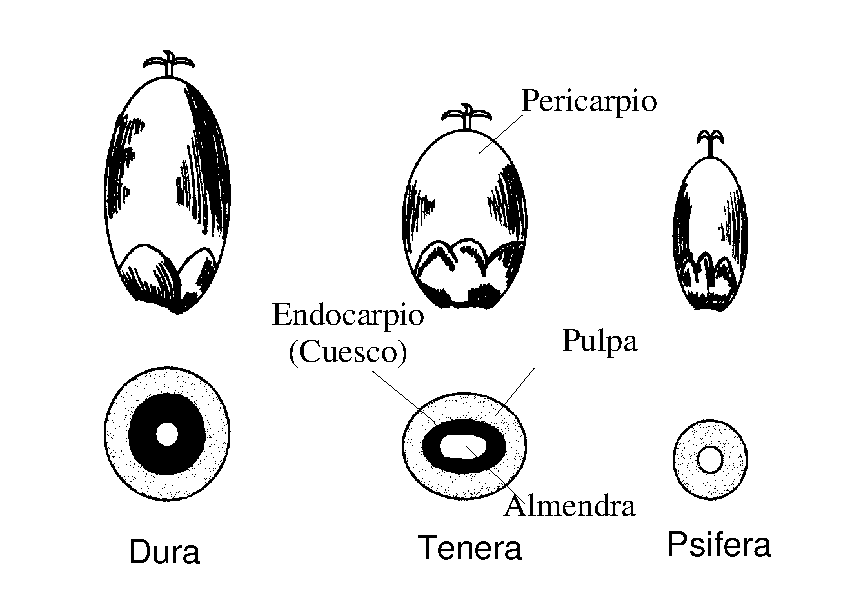
\epsfig{file=Kap3/FrutoSp.eps,scale=1}%
%%\caption{Tipos y partes del fruto de palma de aceite \cite{AG03p,AG04p}.} \label{fig:Fruto}
%%\end{figure}
%
%\section{Ejemplo de presentaci\'{o}n y citaci\'{o}n de tablas y cuadros}
%Para la edici\'{o}n de tablas, cada columna debe llevar su t\'{\i}tulo; la primera palabra se debe escribir con may\'{u}scula inicial y preferiblemente sin abreviaturas. En las tablas y cuadros, los t\'{\i}tulos y datos se deben ubicar entre l\'{\i}neas horizontales y verticales cerradas (como se realiza en esta plantilla).\\
%
%La numeraci\'{o}n de las tablas se realiza de la misma manera que las figuras o ilustraciones, a lo largo de todo el texto. Deben llevar un t\'{\i}tulo breve, que concreta el contenido de la tabla; \'{e}ste se debe escribir en la parte superior de la misma. Para la presentaci\'{o}n de cuadros, se deben seguir las indicaciones dadas para las tablas.\\
%
%Un ejemplo para la presentaci\'{o}n y citaci\'{o}n de tablas (citaci\'{o}n indirecta), se presenta a continuaci\'{o}n:\\
%
%De esta participaci\'{o}n aproximadamente el 60 \% proviene de biomasa
%(Tabla \ref{EMundo1}).
%\begin{center}
%\begin{threeparttable}
%\centering%
%\caption{Participaci\'{o}n de las energ\'{\i}as renovables en el suministro
%total de energ\'{\i}a primaria \cite{AG02i}.}\label{EMundo1}
%\begin{tabular}{|l|c|c|}\hline
%&\multicolumn{2}{c|}{Participaci\'{o}n en el suministro de energ\'{\i}a primaria /\% (Mtoe)\;$\tnote{1}$}\\\cline{2-3}%
%\arr{Region}&Energ\'{\i}as renovables &Participaci\'{o}n de la biomasa\\\hline%
%Latinoam\'{e}rica&28,9 (140)&62,4 (87,4)\\\hline%
%\:Colombia&27,7 (7,6)&54,4 (4,1)\\\hline%
%Alemania&3,8 (13,2)&65,8 (8,7)\\\hline%
%Mundial&13,1 (1404,0)&79,4 (1114,8)\\\hline
%\end{tabular}
%\begin{tablenotes}
%\item[1] \footnotesize{1 kg oe=10000 kcal=41,868 MJ}
%\end{tablenotes}
%\end{threeparttable}
%\end{center}
%
%NOTA: en el caso en que el contenido de la tabla o cuadro sea muy extenso, se puede cambiar el tama\~{n}o de la letra, siempre y cuando \'{e}sta sea visible por el lector.\\
%
%\subsection{Consideraciones adicionales para el manejo de figuras y tablas}
%Cuando una tabla, cuadro o figura ocupa m\'{a}s de una p\'{a}gina, se debe repetir su identificaci\'{o}n num\'{e}rica, seguida por la palabra continuaci\'{o}n.\\
%
%Adicionalmente los encabezados de las columnas se deben repetir en todas las p\'{a}ginas despu\'{e}s de la primera.\\
%
%Los anteriores lineamientos se contemplan en la presente plantilla.\\
%
%\begin{itemize}
%\item Presentaci\'{o}n y citaci\'{o}n de ecuaciones.
%\end{itemize}
%
%La citaci\'{o}n de ecuaciones, en caso que se presenten, debe hacerse como lo sugiere esta plantilla. Todas las ecuaciones deben estar numeradas y citadas detro del texto.\\
%
%Para el manejo de cifras se debe seleccionar la norma seg\'{u}n el \'{a}rea de conocimiento de la tesis  o trabajo de investigaci\'{o}n.\\

\chapter{Contexto Te�rico}
En este cap�tulo se realiza una somera exposici�n acerca de los temas principales y conceptos te�ricos m�s relevantes relacionados con el desarrollo del trabajo, la explicaci�n de algunos conceptos que resultan esenciales para que se pueda entender c�mo se realiza la interacci�n de los elementos que componen al desarrollo que se desea realizar, siendo estos de dos �reas muy diferentes pero como pretende este trabajo demostrar complementarias.\\

Como primera medida se realiza la exposici�n  los principales conceptos de geodesia satelital  referentes  al sistema global de navegaci�n por sat�lite GNSS (Global Navigation Satellite System), posteriormente se presenta el proceso que se pretende analizar m�s a fondo con el procesamiento de datos como es la t�cnica de posicionamiento por punto preciso y para finalizar el cap�tulo una explicaci�n de las herramientas que ser�n evaluadas en la etapa de la arquitectura del sistema en el desarrollo metodol�gico del trabajo.

\section{Sistema GPS (Global Positioning System)}
Se presenta en este �tem una introducci�n a lo que son los aspectos m�s relevantes del sistema de posicionamiento global, como lo son quien fue el que lo financi� y desarrollo, cuantos sat�lites lo componen, la longitud de onda en que transmite la se�ales y sus aplicaciones primarias. con el fin de dar a conocer un peque�o resumen de este sistema antes de entrar en el tema de los datos que este proporciona y el uso de estos.\\

Un resumen muy elemental pero que cumple con el prop�sito de explicar sistema de posicionamiento global (GPS) es el siguiente: Perteneciente al gobierno de los estados unidos, este provee una se�al de uso civil. Esta se�al es transmitida de manera simult�nea por una constelaci�n compuesta de 32 sat�lites, cada uno de estos se transporta sobre una �rbita de 12 horas, generalmente desde cualquier posici�n se puede tener como visibles de 8 a 12 sat�lites del total que componen esta constelaci�n, lo cual es un elemento que facilita la captura de datos en un proceso de obtenci�n de datos con un receptor para el fin de tener observaciones de navegaci�n con la cuales poder trabajar posteriormente y de esta forma que no se presenten rastros de intermitencia en la se�al provocados por una no transmisi�n de datos o p�rdida de calidad en la informaci�n al no haber suficientes sat�lites\cite{GPStkug,baker1963xiith}.\\

Cada uno de los sat�lites transmite una se�al en el espectro electromagn�tico, estas se�ales son propagadas a 1575.42 y 1227.6 MHz, son llamadas $L_{1}$ y $L_{2}$ respectivamente. En la actualidad la se�al civil es ta designada �nicamente a $L_{1}$, la se�al de $L_{2}$ es usada para aplicaciones militares. La se�al civil tiene dos componentes, un c�digo de tiempo y un mensaje de navegaci�n. Por diferenciaci�n del c�digo de tiempo recibido con el c�digo de tiempo interno el receptor es capaz de determinar la distancia, o el rango, que esta se�al ha viajado. Este rango de observaci�n es afectado por errores en el reloj del receptor, por lo que se llama un pseudorango. El mensaje de navegaci�n contiene las efem�rides de sat�lite, las cuales representan un modelo num�rico de la �rbita del sat�lite\cite{GPStkug,GUI2012,baker1963xiith}.

\section{GLONASS}

GLONASS por sus sigla en ruso Global'naya Navigatsionnaya Sputnikovaya Sistema, es similar en sus caracter�sticas t�cnicas al GPS, este es un sistema Ruso que actualmente se encuentra activo, proporciona a la comunidad civil que hace uso de sus datos una precisi�n en cuanto a posicionamiento absoluto relativamente mejor que el sistema GPS, este hecho es debido a la degradaci�n intencionada de la informaci�n denominada Disponibilidad Selectiva (SA - Selective Availability)\cite{GGNASS}.\\

La constelaci�n del sistema GLONASS est� compuesta por 24 sat�lites contenidos en tres planos orbitales, que tienen un nodo ascendente (o inclinaci�n de la orbita como se ve en la Figura (\ref{fig:IncliOrbit})) de 120\textdegree y un argumento en latitud de 15\textdegree. Cada uno de los planos orbitales aloja un total de 8 sat�lites de la constelaci�n espaciados de forma regular, con un argumento en longitud de 45\textdegree. Estos planos est�n inclinados un con respecto al Ecuador cerca de 64.8\textdegree. Los sat�lites de esta constelaci�n se encuentran aproximadamente a una distancia de 19100 Km de la tierra en �rbitas casi circulares, tiene un periodo orbital de 675.8 minutos ( aproximadamente 11 horas y 26 minutos),  esto quiere decir que se garantiza un m�nimo de 5 sat�lites visibles, con los cual se puede concluir que la constelaci�n de GLONASS est� en capacidad de proporcionar una cobertura continua y global para fines de ejecuci�n de observaciones de navegaci�n\cite{GGNASS}.\\

\begin{figure}[!ht]
\centering
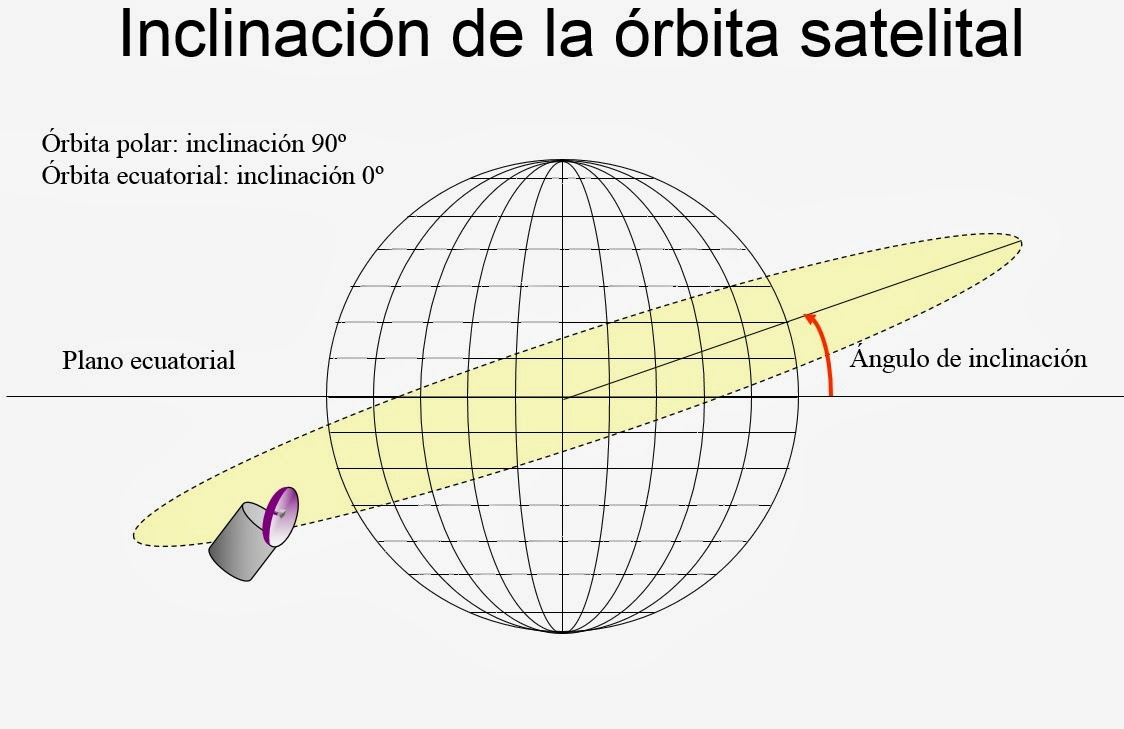
\includegraphics[width=12cm]{Kap3/Fig_Kap3/Inclinacionorbita.jpg} %height=8cm,
\caption[Inclinaci�n Sat�lite]{Inclinaci�n orbital de un sat�lite. Fuente: \href{http://astronomia-fisica-misiones-espaciales.blogspot.com/}{Astronomia Fisica Misiones Espaciales - visto (02-03-2014)}}
\label{fig:IncliOrbit}
\end{figure}

La constelaci�n de sat�lites GLONASS transmite en las bandas $L_{1}$ y $L_{2}$ las cuales est�n aproximadamente distribuidas de la siguiente forma, L1 es transmitida en una longitud de onda que se encuentra entres los 1598.0625 - 1604.25 MHz, mientras que $L_{2}$ lo hace en la longitud aproximada de 1242.9375 - 1247.75 MHz. Por estas bandas GLONASS transmite el c�digo $P$, mientras que el c�digo $C/A$ de momento esta solo en la banda $L_{1}$, pero se pens� que tambi�n est� disponible en la banda $L_{2}$ para uso civil, que con la entrada en funcionamiento de la constelaci�n GLONASS-M en 2005 este hecho se hace realidad, aumentando la calidad de los datos obtenidos en cuanto a mejores prestaciones en precisi�n de los datos y calidad de la se�al\cite{GGNASS,GPStkug,baker1963xiith}.

\section{GNSS}

Sistema global de navegaci�n por sat�lite, en sus siglas en ingles GNSS (Global Navigation Satellite System), es el t�rmino gen�rico est�ndar para sistemas de navegaci�n por sat�lite que proporcionan cobertura global de posicionamiento de manera aut�noma, el cual tiene sus or�genes con GPS de origen militar desarrollado por el departamento de defensa de los Estado Unidos, durante los a�os 70 del siglo XX, que empieza a utilizarse con usos civiles a mediado de los a�os 90\cite{pas10}.\\

GNSS, permite determinar la posici�n (longitud, latitud, altura) y el tiempo, a trav�s de las constelaciones de sat�lites, receptores y vigilancia de la integridad del sistema con el aumento requerido en la operaci�n prevista. (Anexo 10 del Convenio sobre Aviaci�n Civil Internacional, 2006) 
Primera fase (GNSS-1): Formado por los dos sistemas de navegaci�n por sat�lite operativos actuales (el GPS estadounidense y el GLONASS ruso), junto con los sistemas de aumento: SBAS, GBAS, ABAS\cite{TUED}.\\

Segunda fase (GNSS-2): Formado por el nuevo sistema Galileo, el reciente COMPASS chino y las actualizaciones de los actuales GPS y GLONASS\cite{TUED}.

\begin{itemize}
\item Precisi�n: grado de coincidencia entre la posici�n y/o Velocidad estimada o medida con respecto a la Posici�n y/o velocidad real.\\
\item Integridad (incluyendo tiempo hasta alerta): La seguridad de que todas las funciones de un sistema son realizadas dentro de los l�mites operacionales, proporcionando el sistema de navegaci�n las alarmas correspondientes con el tiempo suficiente al usuario cuando el sistema no deba usarse para la navegaci�n o una operaci�n dada.\\
\item Continuidad de servicio: Es la posibilidad de que el sistema de navegaci�n proporcione el servicio sin interrupci�n durante una operaci�n dada.\\
\item Disponibilidad del servicio: Es la posibilidad de que el sistema pueda realizar su funci�n al inicio de una operaci�n dada.
\end{itemize}

\section{Datos RINEX y Efem�rides Precisas SP-3}

El formato de intercambio independiente del receptor como ser�a la traducci�n literal de sus siglas en ingl�s (The Receiver INdependent EXchange), tambi�n llamado RINEX en el �mbito de los profesionales en el �rea de navegaci�n sat�lital y afines. Este formato permite estandarizar los datos para que sea posible por medio de los programas especializados hacer lectura y uso de los mismos.\\

El formato RINEX fue desarrollado por el Servicio Geod�sico Nacional (NGS) en los Estados Unidos y la Universidad de Berna en Suiza. RINEX son realmente tres definiciones de formato que permiten el almacenamiento de observaciones GPS, informaci�n del mensaje de navegaci�n GPS, y datos meteorol�gicos asociados con observaciones GPS. La biblioteca GPSTk contiene clases para leer y escribir datos RINEX en su version 2.1 y 3, de todos los tipos (observados, mensajes de navegaci�n y meteorol�gicos)\cite{GPStkug}.\\

Por otra parte se hace necesaria una definicion del contenido de los ficheros SP-3, los cuales son usados para almacenar informacion referente a las efemerides de los satelites. Usualmente esta informacion esta asociada a las efemerides precisas. La libreria que se usara para el desarrollo de la parte de procesamiento de datos GPSTK, tiene la capacidad de manipular archivos de tipo SP-3a y SP-3-c. El formato SP-3 fue dise�ado originalmente por el Servicio Geod�sico Nacional (NGS) de los Estados Unidos\cite{GPStkug}.

\section{Procesamiento por Punto Preciso}

Precise Point Positioning (PPP) es un m�todo de posicionamiento que utiliza los productos extensamente y f�cilmente disponibles de �rbitas y correcciones de reloj del Sistema Global de Navegaci�n por Sat�lite (GNSS), por ejemplo, obtenidos a trav�s del Servicio Internacional de GNSS\footnote{IGS - \url{http://igs.org} visto el (02-03-2014)}, para realizar el posicionamiento de un punto utilizando tan solo un �nico receptor GNSS.\cite{ppp12,ELPPP2000,ppp02}.\\

En \cite{kouba2001} se dice que el modelo usado por el PPP es a grandes rasgos similar al que utiliza el servicio de posicionamiento est�ndar ofrecido por el GPS. Tambi�n se puede destacar con respecto al procesamiento por punto preciso que el procesamiento de un d�a completo de observaciones est�ticas de alta receptores de frecuencia dual con un software de procesamiento de PPP produce mayor precisi�n posicional hasta nivel de cent�metro, tanto horizontal como verticalmente. Acortar el per�odo de tiempo de observaciones continuas y pasar de modo est�tico a cinem�tico disminuir� la precisi�n. Por ejemplo 6 horas de observaciones cinem�ticas suelen dar precisi�n a nivel de unos pocos cent�metro, mientras que 1 hora de las observaciones da precisi�n a nivel de dec�metro\cite{ppp06}.\\

El algoritmo para procesamiento por punto preciso PPP fue desarrollado para trabajar en base solo a observaciones del sistema GPS. La precisi�n, disponibilidad y fiabilidad de los resultados del PPP sin embargo son bastante dependes del n�mero de sat�lites visibles. Bajo entornos como zonas urbanas en barrancos, monta�as y minas a cielo abierto, por ejemplo, el n�mero de sat�lites GPS visibles es a menudo insuficiente para la determinaci�n de la posici�n\cite{Tsuji2000}. Adem�s, incluso en el �rea abierta donde los sat�lites GPS disponibles son suficientes, la exactitud y la fiabilidad pueden todav�a insuficientes debido a una mala geometr�a satelital PPP. Una posible forma de aumentar la disponibilidad de sat�lites, as� como la fiabilidad de los resultados de posicionamiento es integrar las observaciones GPS y GLONASS. El beneficio de esta integraci�n es evidente sobre todo para aplicaciones en zonas urbanas de dif�cil acceso, monta�a y entornos de miner�a a cielo abierto\cite{ppp07}.\\

Finalmente es necesario agregar que existen algunas diferencias que hacen al procesamiento por punto preciso sea la t�cnica que se selecciono para el desarrollo de este trabajo, como que el PPP difiere de la t�cnica diferencial de GNSS en que para la segunda es necesario tener acceso a observaciones de una o m�s estaciones de referencia con coordenadas conocidas\cite{thomas11}.\\

Adicionalmente como se muestra en la tabla \ref{tab:1} que expresa en forma resumida las diferencias que existen entre los tipos de correcciones usados por la t�cnica de PPP y diferencial respectivamente, esta comparaci�n sirve como punto de partida para la selecci�n de la que se considera la mejor t�cnica de procesamiento para implementar en el desarrollo de la aplicaci�n.


\begin{table}[h!]
\caption[Comparaci�n de los tipos de correcci�n utilizados por la t�cnica PPP y diferencial]{Comparaci�n de los tipos de correcci�n utilizados por la t�cnica PPP y diferencial de posicionamiento. Fuente: Tomado de \cite{ppp12}}
\begin{center}
\begin{tabular}{|l|c|c|}
\hline \rowcolor{gray} Correction Type                           & PPP & Differential GNSS \\ 
\hline \rowcolor{lightgray} Satellite Specific errors                 & \checkmark & \texttimes \\ 
\hline Precise satellite clock corrections       & \checkmark &  \\ 
\hline Satellite antenna phase centre offset     & \checkmark & \checkmark \\ 
\hline Satellite antenna phase centre variations & \checkmark & \checkmark \\ 
\hline Precise satellite orbits                  & \checkmark & \checkmark/\texttimes \\ 
\hline Group delay differential                  & \checkmark(only L1) & \texttimes \\ 
\hline Relativity                                & \checkmark & \texttimes \\ 
\hline Satellite antenna phase wind-up error     & \checkmark & \texttimes \\ 
\hline \rowcolor{lightgray} Receiver Specific Errors                  &  &  \\ 
\hline Receiver antenna phase centre offset      & \checkmark & \checkmark \\ 
\hline Receiver antenna phase centre variations  & \checkmark & \checkmark \\ 
\hline Receiver antenna phase wind-up            & \checkmark & \texttimes \\ 
\hline \rowcolor{lightgray} Geophysical Models                        &  &  \\ 
\hline Solid earth tide displacements            & \checkmark & \texttimes \\ 
\hline Ocean loading                             & \checkmark & \texttimes \\ 
\hline Polar tides                               & \checkmark & \texttimes \\ 
\hline Plate tectonic motion                     & \checkmark & \texttimes \\ 
\hline \rowcolor{lightgray} Atmospheric Modelling                     &  &  \\ 
\hline Troposphere                               & \checkmark & \checkmark \\ 
\hline Ionosphere                                & \checkmark(only L1) & \texttimes \\ 
\hline 
\end{tabular} 
\end{center}
\label{tab:1}
\end{table}

\section{GPSTK (GPS ToolKit)}

El objetivo principal del proyecto de desarrollo de GPSTk es proporcionar una librer�a de c�digo abierto y adicionalmente a ella un conjunto de aplicaciones disponibles en la comunidad de personas que hacen uso de datos correspondientes a navegaci�n por sat�lite, con el fin de facilitar a los investigadores un libre desempe�o para centrarse en la investigaci�n y no en la codificaci�n de bajo nivel para poder realizar el procesamiento de sus datos\cite{GPStkug}.\\

Los usuarios de GPS emplean pr�cticamente todas las arquitecturas de c�mputo y versiones de sistemas operativos. Por lo tanto el dise�o de la librer�a GPSTk tiene que dar como resultado un conjunto de software tan independiente de la plataforma como sea posible. La independencia de la plataforma se consigue a trav�s del uso del lenguaje de programaci�n est�ndar ISO C++. Los principios de la programaci�n orientada a objetos que son utilizados en GPSTk se usan principalmente con el fin de asegurarse de que el c�digo es modular, extensible y mantenible\cite{GPStkug}.\\

El conjunto de herramientas GPSTk consta de una biblioteca n�cleo, bibliotecas auxiliares, y un conjunto de aplicaciones. GPSTk tambi�n proporciona una amplia gama de funciones que resuelven problemas de procesamiento asociados con GPS, as� como el procesamiento utilizando formatos est�ndar: como RINEX. Las bibliotecas son la base de las aplicaciones m�s avanzadas que son distribuida de manera conjunta con el conjunto que conforma GPSTk\cite{GPStkug}.\\

El conjunto de software que conforma GPSTk es patrocinado por el Laboratorio Espacial y de Geof�sica, que hace parte de los Laboratorios de Investigaci�n Aplicada de la Universidad de Texas en Austin. GPSTk es el producto de la investigaci�n realizada en GPS ARL: UT desde antes del primer sat�lite lanzado en 1978, es el esfuerzo conjunto de muchos ingenieros de software y cient�ficos. En 2003, el personal de investigaci�n en ARL: UT decidi� promover como c�digo abierto gran parte de su software de procesamiento para GPS como producto de ese evento nace GPSTk\cite{GPStkug}.

\section{Ruby on Rails}

Ruby on Rails, generalmente abreviado como Rails, es un completo framework de desarrollo para aplicaciones web, escrito en el lenguaje de programaci�n Ruby. el uso de este framework depende mucho de la experiencia que se tenga en el �mbito de la programaci�n. Este framework tiene que ser visto desde el contexto del desarrollo de aplicaciones web si realmente se quiere apreciar su potencialidad\cite{lenz08}.\\

En el desarrollo  de este trabajo se pretende realizar una aplicaci�n que siga el modelo vista controlador, este es el mismo que utiliza ruby on rails, por ese motivo es que se ha hecho la elecci�n del mismo, que en este caso va a desempe�ar la labor de controlador. Desempe�ando la funci�n de Recibir los datos y enviarlos para que sean procesados, luego de este proceso los datos los enviara v�a correo electr�nico a el usuario que se realice la solicitud, de esta forma el usuario tendr� procesados sus datos por medio de la t�cnica de procesamiento por punto preciso y sin antes haber tenido que instalar un programa especializado para este tipo de labor.

\section{Bootstrap}

Bootstrap es un producto de c�digo abierto desarrollado por Mark Otto y Jacob Thornton, quienes cuando fue hicieron el primer lanzamiento de este producto a�n eran empleados de twitter. Hab�a una necesidad de estandarizar el conjunto de herramientas que eran usadas por los ingenieros en toda la compa��a para el desarrollo de la  interfaz\cite{lenz08}.\\

En forma m�s expl�cita Bootstrap es un conjunto de estilos y funciones que permiten un desarrollo �gil de la interfaz de un sitio web, este concepto permite poder hacer ese desarrollo usando funcionalidades que actualmente son est�ndar en esta �rea del desarrollo web. Este aspecto permite que quien realiza su aplicaci�n pueda prestar los servicios de la misma para diferentes tipos de dispositivos, no solo computadores de escritorio sino tambi�n tabletas y dispositivos m�viles.\\

Por las razones expuestas anteriormente es que se recurre a esta tecnolog�a como herramienta para realizar el desarrollo de la interfaz web de la aplicaci�n que sera el producto del proyecto.

\section{Antecedentes}

En la actualidad se ha dado mucha importancia a las aplicaciones web, en vista al futuro pr�ximo donde la mayor�a de los procesos van a estar orientados a la web, muchos de los grandes productores de software han ido tomando parte en la red para distribuir sus servicios de esta manera, en ese sentido las aplicaciones relacionadas con el concepto de procesamiento de datos no has sido la excepci�n y muchos distribuidores y entidades relacionadas con el tema ya empezaron su producci�n.\\

Uno de los casos m�s notables lo propone la Divisi�n de navegaci�n Geod�sica del departamento de recursos naturales de Canad�. Lanzando en Noviembre de 2003 dentro del CSRS-PPP que por sus siglas Canadian Spatial Reference System, como un servicio web\footnote{CSRS-PPP - \url{http://webapp.geod.nrcan.gc.ca/geod/tools-outils/ppp.php} - Visto el (02-03-2014)} que permite este tipo de procesamiento por punto preciso, una imagen de la aplicaci�n se puede ver en la Figura(\ref{fig:CSRSPPP}).\\

\begin{figure}[!ht]
\centering
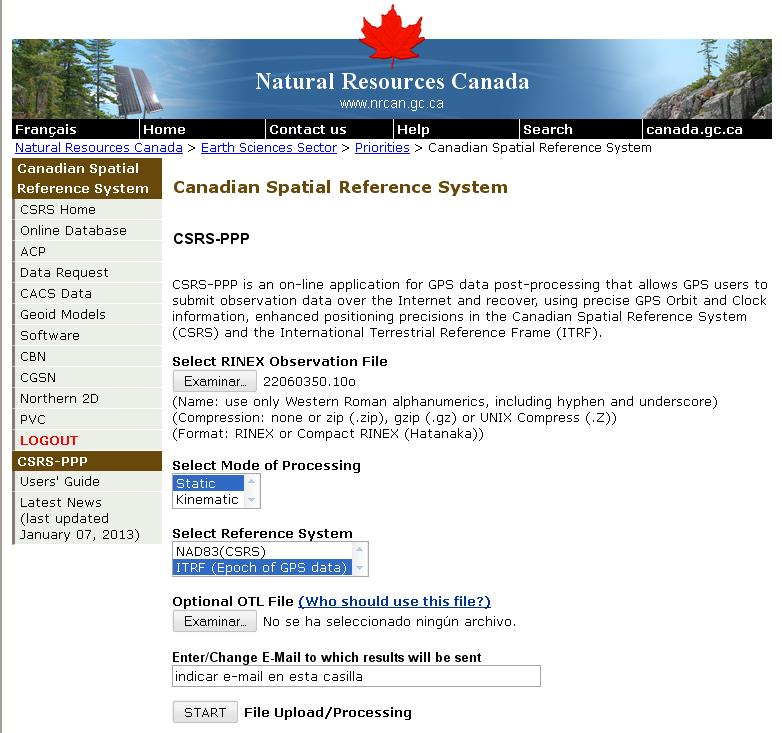
\includegraphics[width=11cm]{Kap3/Fig_Kap3/CSRSPPP.JPG} %height=8cm,
\caption[Aplicaci�n de PPP del CSRS]{Aplicaci�n web PPP del CSRS. Fuente:\href{http://webapp.geod.nrcan.gc.ca/geod/tools-outils/ppp.php}{Captura web CSRS-PPP - Visto el (02-03-2014)}}
\label{fig:CSRSPPP}
\end{figure}

De la misma forma el IBGE Instituto Brasileiro de Geografia e Estat�stica pone en funcionamiento su servicio de procesamiento de datos en l�nea\footnote{IBGE PPP (02-03-2014)- \url{http://www.ppp.ibge.gov.br/ppp.htm}}, el cual se muestra en la Figura(\ref{fig:IBGEPPP}) y funciona a partir de un archivo que el usuario sube a la red, el cual posteriormente es procesado y el producto de este procesamiento es puesto a disposici�n para que el usuario lo descargue.\\

\begin{figure}[!ht]
\centering
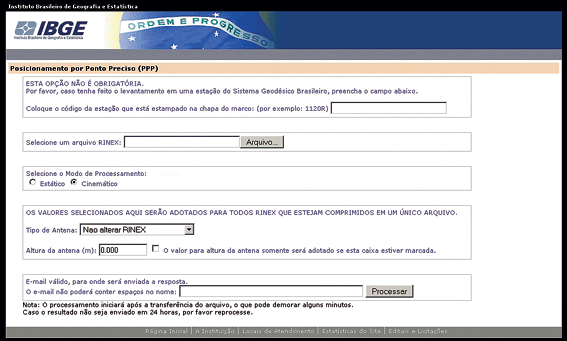
\includegraphics[width=12cm]{Kap3/Fig_Kap3/IBGEPPP.png} %height=8cm,
\caption[Aplicaci�n de PPP del IBGE]{Aplicaci�n web PPP del IBGE. Fuente:\href{http://www.ppp.ibge.gov.br/ppp.htm}{Captura web PPP del IBGE - Visto el (02-03-2014)}}
\label{fig:IBGEPPP}
\end{figure}

Otro de los casos de �xito a destacar en cuanto a las aplicaciones que prestan el servicio de posicionamiento por punto preciso es el desarrollado en el departamento de ingenier�a de geodesia y geom�tica en la University of New Brunswick, ubicada en Fredericton - Canad�. Esta Aplicaci�n se llama GAPS\footnote{GAPS PPP (02-03-2014) - \url{http://gaps.gge.unb.ca/About.html}}, por sus siglas en ingles GPS Analysis and Positioning Software.\\

Al ser una aplicaci�n de tipo web tambi�n es un gran antecedente para el trabajo que se desea desarrollar, se incluye en la Figura (\ref{fig:GAPSPPP}) una vista de la pagina web en la que se aloja la aplicaci�n.\\

\begin{figure}[!ht]
\centering
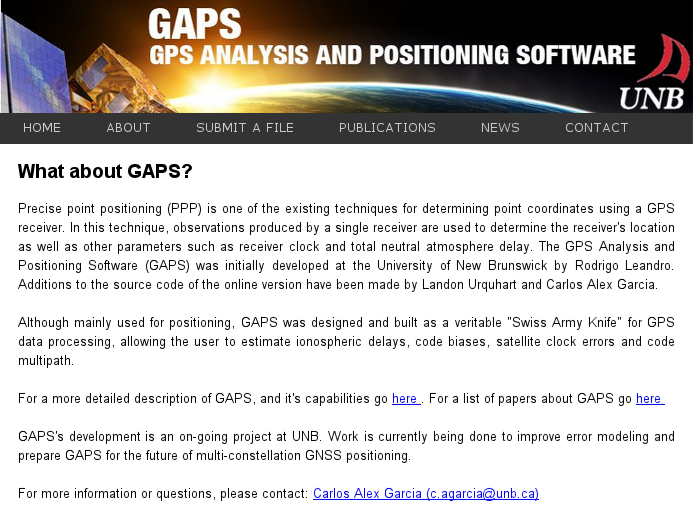
\includegraphics[width=12cm]{Kap3/Fig_Kap3/GAPSPPP.png} %height=8cm,
\caption[Aplicaci�n de PPP del Dep Geodesy and Geomatics]{Aplicaci�n web PPP del Departamento de ingenier�a de geodesia y geom�tica en la University of New Brunswick. Fuente:\href{http://gaps.gge.unb.ca/About.html}{Captura web GAPS PPP - Visto el (02-03-2014)}}
\label{fig:GAPSPPP}
\end{figure}

En el campo del procesamiento de datos satelitales para determinar la posici�n de un punto, la NASA no pod�a quedarse atr�s y tambi�n implementa su aplicaci�n para procesamiento de datos, denominada  Automatic Precise Positioning Service\footnote{NASA PPP (02-03-2014) - \url{http://apps.gdgps.net/apps_file_upload.php}} de la cual se adjunta una vista en la Figura(\ref{fig:NASAPPP}).\\

\begin{figure}[!ht]
\centering
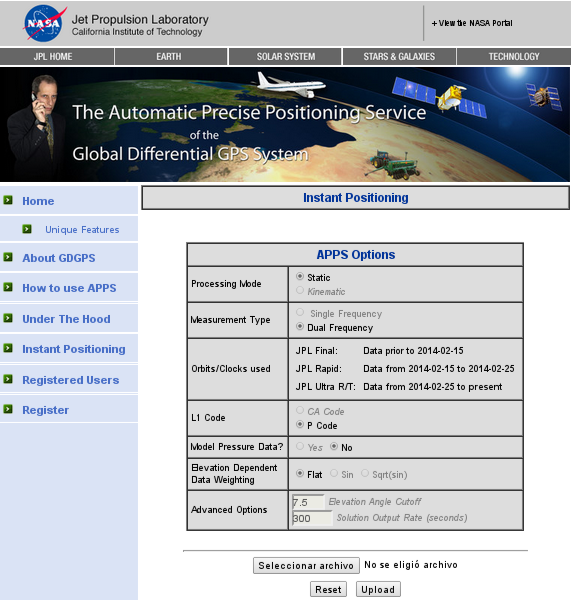
\includegraphics[width=12cm]{Kap3/Fig_Kap3/NASAPPP.png} %height=8cm,
\caption[Aplicaci�n de PPP de la NASA]{Aplicaci�n web PPP desarrollado por la NASA. Fuente:\href{http://apps.gdgps.net/apps_file_upload.php}{Captura web NASA PPP - Visto el (02-03-2014)}}
\label{fig:NASAPPP}
\end{figure}

Como estas aplicaciones hay muchas, tanto de proveedores p�blicos como de empresas privadas. Lo que hace innovador este proyecto es ser el primero que se realiza de este estilo en un pa�s de habla hispana y adem�s que se realiza bajo la filosof�a del software libre, donde las personas que deseen pueden descargar el c�digo y contribuir con el programa para que este con el futuro pueda prestar mayores servicios a los relacionados en este proyecto.\\ 

Para finalizar este item del capitulo tambi�n se destaca el uso de herramientas que estos proyectos anteriormente mencionados no ha puesto en practica en su desarrollo. Como son la extensi�n de ruby llamada rails para desarrollar las vistas y el controlador de la aplicaci�n, bootstrap para el dise�o de la interfaz de usuario y la biblioteca para desarrollo de aplicaciones satelitales GPSTK,  la cual esta escrita en lenguaje C++.\\

Es esperado realizar un trabajo que sea medianamente parecido a todos estos grandes desarrollos que preceden a la aplicaci�n de la cual es tema este proyecto, pero se es consciente que esta sera desarrollada por una sola persona al principio y por su licencia es posible que en el futuro se unan mas desarrolladores para poder dar un mejor soporte a la misma.\\
\chapter{Dise�o Metodol�gico}

El proyecto es concebido como una oportunidad para poner en pr�ctica los conocimientos obtenidos en algunas de las diferentes asignaturas vistas en el transcurso de la carrera, haciendo uso de el conocimiento proporcionado por estas como la herramienta fundamental para poder realizar la estructura de una aplicaci�n que pretende dar soluci�n a una problem�tica que se presenta en la actualidad, como es el uso de software propietario y de dif�cil acceso en el �rea del post procesamiento de datos Rinex. Por tal motivo es indispensable hacer una recopilaci�n de las dificultades m�s conocidas que se presentan al momento de post-procesar datos satelitales por el m�todo de punto preciso. A esta parte en el desarrollo de la  metodolog�a del proyecto haciendo alusi�n al desarrollo de software se de denominar� seg�n los est�ndares de ahora en adelante la etapa de \textit{Definici�n de Requerimientos}, esta definici�n es ampliamente usada en \cite{Moore2002,IEEEStd830,Juristo2007}.\\

\begin{figure}[H]
\centering
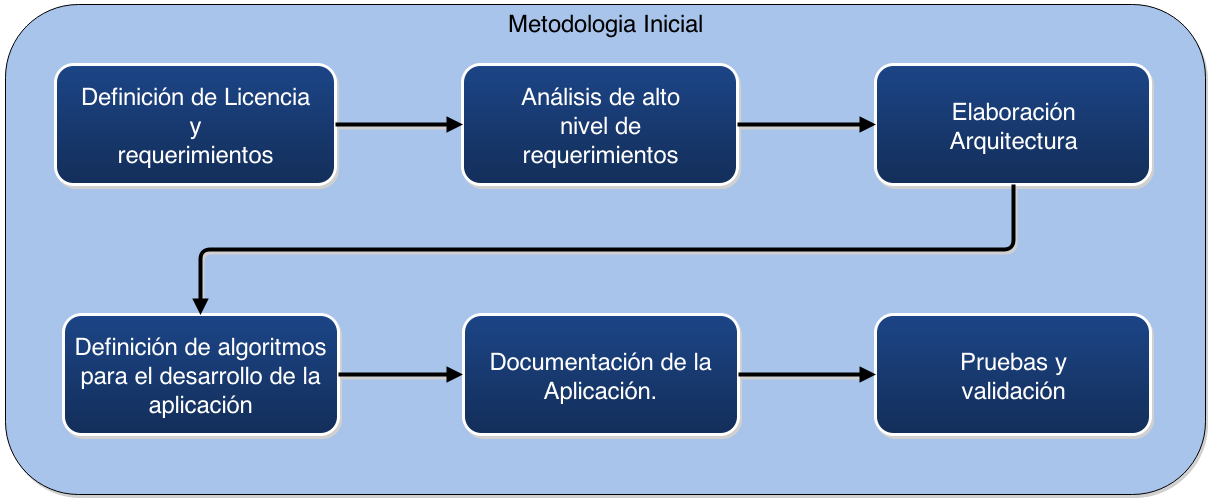
\includegraphics[width=16cm]{Kap3/Fig_Kap3/MetodologiaProyecto.png} %height=8cm,
\caption[Metodolog�a del Proyecto]{Gr�fico Metodolog�a del Proyecto}
\label{fig:MetProy}
\end{figure}

Por definici�n de requerimientos se entiende la etapa o el proceso que constituye la principal fuente de informaci�n a partir de la cual se dise�a, implementa y prueba el sistema\cite{IEEEStd830}. Tiende a ser uno de los procesos m�s delicados en el desarrollo de un proyecto, esta etapa no se realiza en su totalidad al principio del proyecto sino que es incremental aun cuando el proyecto ya ha comenzado a desarrollarse.\\

En otros aspectos tambi�n es importante tener en cuenta el dise�o de lo que ser� definir la \textit{Elaboraci�n de Arquitectura del Sistema}\cite{jacobson2004,serrano2010,vogel2011}. la que tendr� que ser acorde con los requerimientos primarios del sistema para que pueda dar soluci�n a estos y de esta forma se cumpla con el prop�sito de la aplicaci�n. Es indispensable que para que se tenga coherencia con el t�tulo del proyecto que los actores involucrados en la arquitectura pertenezcan a la misma familia de software que se pretende desarrollar, tanto las librer�as de procesamiento de datos satelitales como las librer�as y lenguajes para el desarrollo de la aplicaci�n y la interfaz web.\\

la etapa posterior a la definici�n de la arquitectura del sistema es el \textit{Dise�o y Desarrollo del Sistema}\cite{vogel2011}. Que para el caso de este proyecto ha sido denominado Definici�n de algoritmos y Desarrollo de la Aplicaci�n, estando definidas las herramientas que compondr�n el sistema y los niveles en los cuales van a actuar cada una de estas se procede a establecer un dise�o preliminar y selecci�n tanto de los algoritmos matem�ticos como de programaci�n con el fin de empezar la etapa de desarrollo de la aplicaci�n.\\ 

Dentro la etapa de dise�o y desarrollo se establece como prioridad el uso de patrones de dise�o de software, para que el desarrollo de la aplicaci�n est� acorde con las caracter�sticas que deben seguir los patrones de desarrollo de software tales como: que sea comprobable la efectividad del desarrollo en la resoluci�n del problema para el cual se dise��, como tambi�n el hecho de que el desarrollo debe ser reutilizable para que el uso o implementaci�n de este en otros problemas similares sea posible aun bajo distintas circunstancias\cite{deitel2004,gamma2002,lopez2004}.\\

Por �ltimo pero no menos importante esta la etapa de \textit{Pruebas y Validaci�n} de la aplicaci�n, la cual tiene como prop�sito realizar una evaluaci�n al desarrollo de la aplicaci�n y de esta forma establecer si esta cumple o no con los los objetivos propuestos. En la etapa de pruebas se deben proponer una hip�tesis que posteriormente ser�n las que nos dar�n la medida de bondad para el desarrollo realizado. Tambi�n se debe tener en cuenta un modelo general de pruebas para poder comparar los resultados obtenidos con los que existes y de esta forma poder corroborar la valides de las hip�tesis propuestas.\\

Es necesario tener en cuente que para las pruebas que de debe realizar estas de manera ordenada y lo m�s precisa posible, para que en caso tal que se presenten errores se pueda reportar estos de forma f�cil tanto en la etapa de identificaci�n como en la de soluci�n de los mismos. Como desde el principio se pretende que para el desarrollo de la aplicaci�n se aplique un modelo que sea iterativo e incremental esta etapa de pruebas debe estar lo mejor dise�ada posible para que las iteraciones del sistema no afecten el desarrollo de toda la aplicaci�n.\\

La etapa de documentaci�n no es incluida dentro de las etapas maestras por que no es de gran relevancia en el desarrollo te�rico del proyecto, pero si se coloca en el documento porque es esencial para el desarrollo practico del proyecto.\\

\section{Definici�n de Requerimientos y licencia de la Aplicaci�n}

Esta secci�n generalmente suele denominarse tambi�n Especificaci�n de requisitos de software, la cual esta definida por el est�ndar de 830 de la IEEE\cite{IEEEStd830}. en el cual se presenta el procedimiento que se debe realizar para poder desarrollar un buen documento de requerimientos, el cual es esencial y se quiere desarrollar una buena aplicaci�n.\\

El documento de requerimientos seg�n el est�ndar de la IEEE debe estar compuesto por un m�nimo de items, los cuales se pueden ver de forma reducida en la Tabla(\ref{tab:2}).\\

\begin{table}[h!]
\begin{center}
\begin{tabular}{|l|}
\hline \textbf{Documento de Requerimientos} \\
1. Introducci�n \\
1.1 Prop�sito \\
1.2 Alcance \\
1.3 Definiciones, siglas, y abreviaciones \\
1.4 Referencias \\
1.5 Apreciaci�n global \\
2. Descripci�n global \\
2.1 Perspectiva del producto \\
2.2 Funciones del producto \\
2.3 Caracter�sticas del usuario \\
2.4 Restricciones \\
2.5 Atenci�n y dependencias \\
3. Los requisitos espec�ficos \\
 Ap�ndices \\
 Indice \\ 
\hline 
\end{tabular} 
\end{center}
\caption[Componentes est�ndar IEEE 830]{Componentes m�nimos del Documento de requerimientos definido por el est�ndar IEEE 830\cite{IEEEStd830}}
\label{tab:2}
\end{table}


Para esta etapa de la metodolog�a se pretende realizar este documento de requerimientos definido por el est�ndar de la IEEE\cite{IEEEStd830}, pero que resulte acorde a la aplicaci�n objetivo de este proyecto.\\

%\section{An�lisis de alto Nivel de Requerimientos}

\section{Elaboraci�n de Arquitectura}

En el �mbito del desarrollo de software al proceso inicial de dise�o que identifica los subsistemas y establece un marco para el control y comunicaci�n de los subsistemas se llama dise�o arquitect�nico. El resultado de este proceso de dise�o es una descripci�n de la arquitectura de software\cite{sommerville2005}. Casi siempre la etapa de dise�o es confundida y en algunos casos combinada con la con la ``etapa de Definici�n de Requerimientos", pero aun cuando tienen algunas cosas que se pueden llegar a tomar como comunes a ambas etapas convienen mantener la de dise�o mas estrechamente ligada a la arquitectura del software.\\

Enti�ndase por \textit{Arquitectura de Software} a la representaci�n de alto nivel de la estructura de un sistema o aplicaci�n, que describe las partes que la integran, las interacciones entre ellas, los patrones que supervisan su composici�n, y las restricciones presentes a la hora de aplicar estos patrones\cite{salavert2000}.\\

Entendiendo estos dos importantes conceptos previos ahora se puede decir que esta parte del proyecto sera en la cual se realice el dise�o de alto nivel de la aplicaci�n. Teniendo en cuenta las entidades que ser�n parte de la aplicaci�n, como debe efectuarse la comunicaci�n entre estas partes, si las mismas deben seguir patrones previamente definidos o si se desarrollaran algunos nuevos para tal fin, finalmente como se van al organizar las entidades y su representaci�n gr�fica para facilitar el desarrollo de la aplicaci�n.\\

Es importante tambi�n tener en cuenta que si en la etapa anterior se hace una exhaustiva labor al definir los requerimientos esta etapa no sera tan compleja, dado que dependiendo de la forma como se tengan los requerimientos se puede implementar una arquitectura de software ya definida.\\

\section{Definici�n de algoritmos y Desarrollo de la Aplicaci�n}

Es esencial al desarrollar una aplicaci�n el conocer los algoritmos matem�ticos que esta va a implementar. Para este proyecto no es la excepci�n, lo primero que se debe hacer en esta etapa es una revisi�n bibliogr�fica acerca del desarrollo te�rico para algoritmo de procesamiento tentativamente propuesto en el desarrollo del proyecto.\\

Es de suma importancia la explicaci�n del desarrollo matem�tico y finalmente su modelado computacional para transformarlo de un algoritmo matem�tico a uno de computaci�n, el cual pueda ser escrito en un lenguaje de programaci�n para que finalmente pueda ser interpretado por el computador.\\

Realizada la identificaci�n y explicaci�n del o los algoritmos debe empezar a desarrollarse la aplicaci�n y seg�n los lineamientos de la arquitectura de software\cite{salavert2000} a crear los patrones y las relaciones entre estos y las dem�s partes de la aplicaci�n.

\section{Documentaci�n de la Aplicaci�n}

Suele suceder que algunos desarrollos no est�n acompa�ados de una buena documentaci�n, lo cual implica que el software dependiendo el caso puede tornarse dif�cil de comprender, solo utilizable por aquellos quienes los desarrollaron y aun mas importante dif�cil de modificar. Para evitar todos estos inconvenientes es necesario definir un proceso de documentaci�n muy bien estructurado y acorde al proyecto\cite{tate1988}.\\

Dado que es un proceso tedioso (menos creativo) el de documentar la aplicaci�n es necesario que cumpla por lo menos con las caracter�sticas m�nimas porque es esencial para el mantenimiento de la aplicaci�n. La documentaci�n debe describir la manera de usar el programa, las razones que motivaron la creaci�n del programa, las t�cnicas usadas para el desarrollo del mismo y cualquier aspecto que no sea muy claro en el desarrollo\cite{munoz2010}.\\


\section{Pruebas y Validaci�n}

Para la realizaci�n de la etapa de pruebas sera necesario comparar los resultados obtenidos con la aplicaci�n desarrollada y algunas de las alternativas similares que se listaron en el apartado de antecedentes, con el fin de poder hacer una evaluaci�n comparativa con respecto a otras aplicaciones que tienen una mayor trayectoria en el procesamiento de datos RINEX.\\

Precisamente para poder hacer efectiva la etapa de pruebas y validaci�n de los resultados obtenidos se hace necesario definir un procedimiento est�ndar que permita hacer la comparaci�n de la forma mas imparcial posible y que evalu� las mismas capacidades en cada uno de los casos. Todo esto con el fin de hacer la comparaci�n de la mejor manera posible.\\

Para el caso que compete a este proyecto se ha definido un proceso que se puede definir como lo mas sencillos posible en el cual intervienen los factores mas relevantes en el procesamiento de datos satelitales y se ha realizado el diagrama que se muestra en la Figura(\ref{fig:ProcPrueba}). El cual se llamara \textit{Diagrama del Proceso de Pruebas y Validaci�n} y sera el punto de control para las pruebas y validaci�n de resultados de la aplicaci�n desarrollada.\\
\begin{figure}[H]
\centering
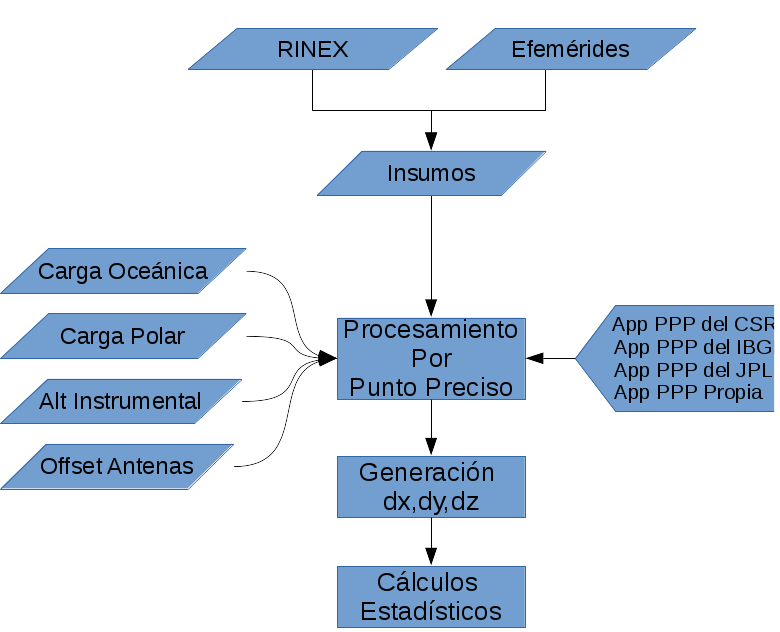
\includegraphics[width=14cm]{Kap4/procesamientotesis.png} %height=8cm,
\caption[Proceso de Pruebas y Validaci�n]{Diagrama del Proceso de Pruebas y Validaci�n}
\label{fig:ProcPrueba}
\end{figure}

Como se puede ver en el Diagrama de la Figura (\ref{fig:ProcPrueba}) se tomaran como datos de entrada unos archivos Rinex cualquiera y las efem�rides correspondientes a la fecha de toma de esos datos, estos archivos van a constituir los insumos de pruebas. Sumado a estos estar�n los modelos que tienen informaci�n que mejora la precisi�n de los datos debido al algoritmo que se pretende utilizar, estos son el modelo de carga oce�nica y el modelo de carga polar acordes a los datos, tambi�n la altura instrumental y finalmente el offset de la antena del equipo.
\newpage
\section{Cronograma de Actividades}

A continuaci�n se muestran las actividades que deben ser desarrolladas para la ejecuci�n del proyecto, ordenadas en una tabla (\ref{fig:Act}) y su respectivo gr�fico de Gantt (\ref{fig:Gantt}). 

\begin{figure}[H]
\centering
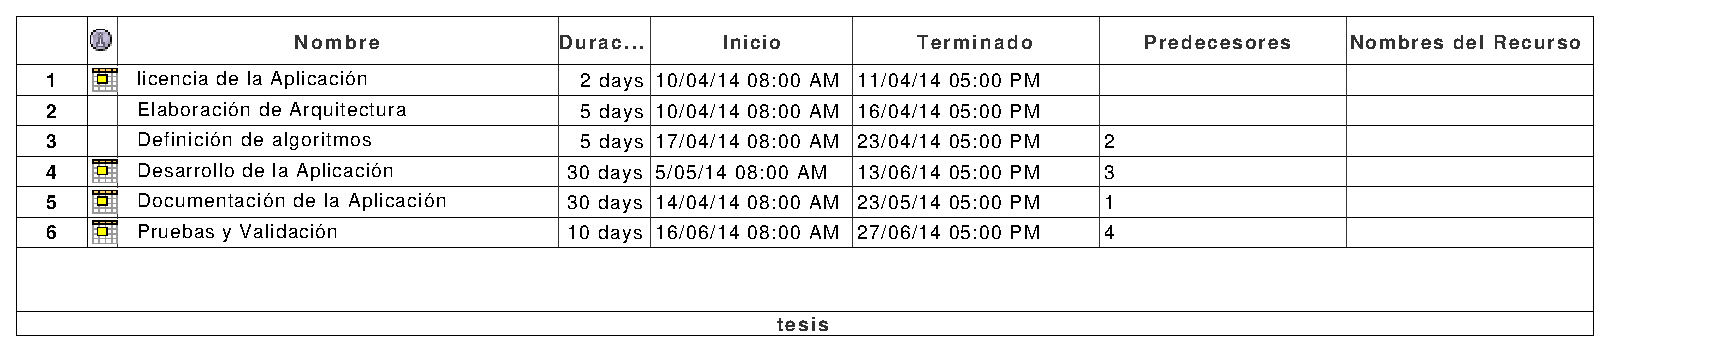
\includegraphics[width=18cm]{Kap5/tesis_crono_tabla.pdf} %height=8cm,
\caption[Gr�fico tabular de Actividades]{Tabla cronograma de las actividades del proyecto,}
\label{fig:Act}
\end{figure}

\begin{figure}[H]
\centering
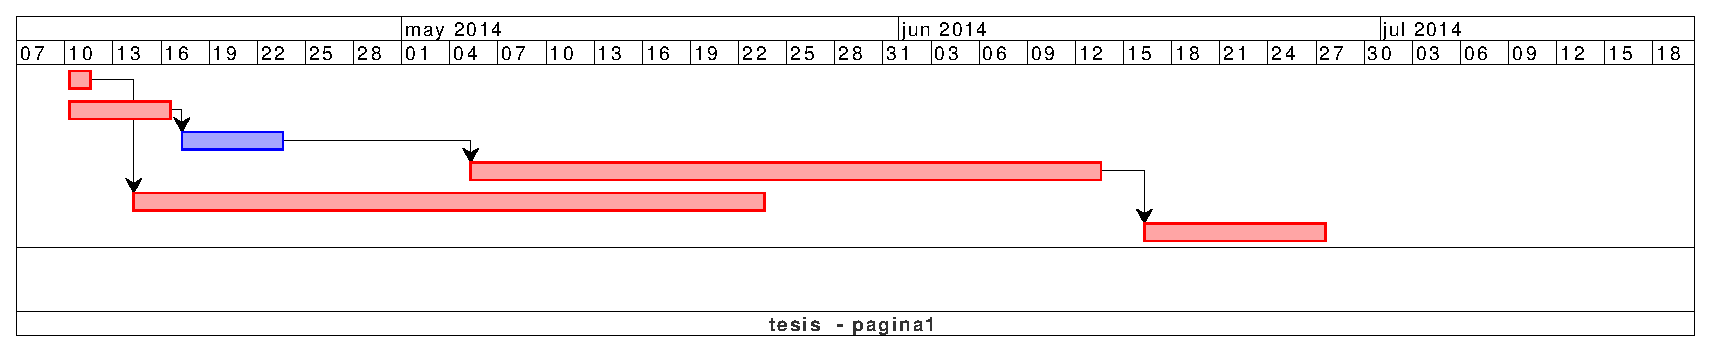
\includegraphics[width=17cm]{Kap5/tesis_crono_gant.pdf} %height=8cm,
\caption[Diagrama Gantt Actividades]{Gr�fico gantt de las actividades del proyecto,}
\label{fig:Gantt}
\end{figure}
%\chapter{Conclusiones y recomendaciones}
\section{Conclusiones}
Las conclusiones constituyen un cap\'{\i}tulo independiente y presentan, en forma l\'{o}gica, los resultados de la tesis  o trabajo de investigaci\'{o}n. Las conclusiones deben ser la respuesta a los objetivos o prop\'{o}sitos planteados. Se deben titular con la palabra conclusiones en el mismo formato de los t\'{\i}tulos de los cap\'{\i}tulos anteriores (T\'{\i}tulos primer nivel), precedida por el numeral correspondiente (seg\'{u}n la presente plantilla).\\

\section{Recomendaciones}
Se presentan como una serie de aspectos que se podr\'{\i}an realizar en un futuro para emprender investigaciones similares o fortalecer la investigaci\'{o}n realizada. Deben contemplar las perspectivas de la investigaci\'{o}n, las cuales son sugerencias, proyecciones o alternativas que se presentan para modificar, cambiar o incidir sobre una situaci\'{o}n espec\'{\i}fica o una problem\'{a}tica encontrada. Pueden presentarse como un texto con caracter\'{\i}sticas argumentativas, resultado de una reflexi\'{o}n acerca de la tesis o trabajo de investigaci\'{o}n.\\

%\begin{appendix}
\chapter{Anexo: Figuras del �rbol de Objetivos y El �rbol de Problemas}\label{AnexoA}
\begin{figure}[!ht]
\centering
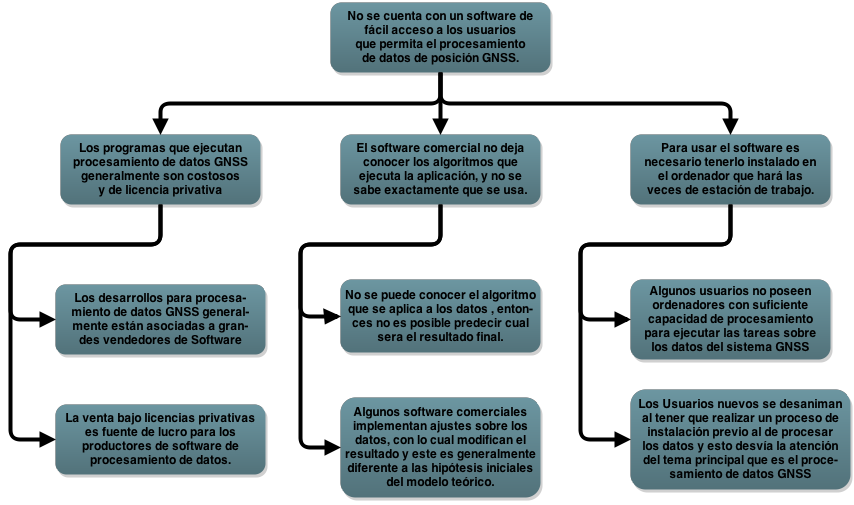
\includegraphics[width=16cm]{Kap3/Fig_Kap3/ArboldeProblemas.png} %height=8cm,
\caption[�rbol de Problemas]{Gr�fica del �rbol de Problemas}
\label{fig:ArProblem}
\end{figure}

\begin{figure}[!ht]
\centering
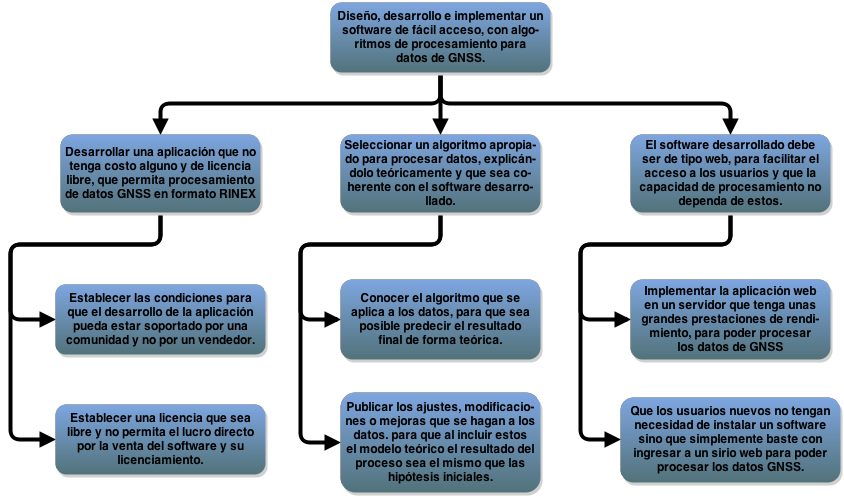
\includegraphics[width=16cm]{Kap3/Fig_Kap3/ArboldeObjetivos.png} %height=8cm,
\caption[�rbol de Objetivos]{Gr�fica del �rbol de Objetivos}
\label{fig:ArObjetivos}
\end{figure}

%\chapter{Anexo: Nombrar el anexo B de acuerdo con su contenido}
%A final del documento es opcional incluir \'{\i}ndices o glosarios. \'{E}stos son listas detalladas y especializadas de los t\'{e}rminos, nombres, autores, temas, etc., que aparecen en el mismo. Sirven para facilitar su localizaci\'{o}n en el texto. Los \'{\i}ndices pueden ser alfab\'{e}ticos, cronol\'{o}gicos, num\'{e}ricos, anal\'{\i}ticos, entre otros. Luego de cada palabra, t\'{e}rmino, etc., se pone coma y el n\'{u}mero de la p\'{a}gina donde aparece esta informaci\'{o}n.\\
%
%\chapter{Anexo: Nombrar el anexo C de acuerdo con su contenido}
%MANEJO DE LA BIBLIOGRAF\'{I}A: la bibliograf\'{\i}a es la relaci\'{o}n de las fuentes documentales consultadas por el investigador para sustentar sus trabajos. Su inclusi\'{o}n es obligatoria en todo trabajo de investigaci\'{o}n. Cada referencia bibliogr\'{a}fica se inicia contra el margen izquierdo.\\
%
%La NTC 5613 establece los requisitos para la presentaci\'{o}n de referencias bibliogr\'{a}ficas citas y notas de pie de p\'{a}gina. Sin embargo, se tiene la libertad de usar cualquier norma bibliogr\'{a}fica de acuerdo con lo acostumbrado por cada disciplina del conocimiento. En esta medida es necesario que la norma seleccionada se aplique con rigurosidad.\\
%
%Es necesario tener en cuenta que la norma ISO 690:1987 (en Espa\~{n}a, UNE 50-104-94) es el marco internacional que da las pautas m\'{\i}nimas para las citas bibliogr\'{a}ficas de documentos impresos y publicados. A continuaci\'{o}n se lista algunas instituciones que brindan par\'{a}metros para el manejo de las referencias bibliogr\'{a}ficas:\\
%
%\begin{center}
%\centering%
%\begin{tabular}{|p {7.5 cm}|p {7.5 cm}|}\hline
%\arr{Instituci\'{o}n}&Disciplina de aplicaci\'{o}n\\\hline%
%Modern Language Association (MLA)&Literatura, artes y humanidades\\\hline%
%American Psychological Association (APA)&Ambito de la salud (psicolog\'{\i}a, medicina) y en general en todas las ciencias sociales\\\hline
%Universidad de Chicago/Turabian &Periodismo, historia y humanidades.\\\hline
%AMA (Asociaci\'{o}n M\'{e}dica de los Estados Unidos)&Ambito de la salud (psicolog\'{\i}a, medicina)\\\hline
%Vancouver &Todas las disciplinas\\\hline
%Council of Science Editors (CSE)&En la actualidad abarca diversas ciencias\\\hline
%National Library of Medicine (NLM) (Biblioteca Nacional de Medicina)&En el \'{a}mbito m\'{e}dico y, por extensi\'{o}n, en ciencias.\\\hline
%Harvard System of Referencing Guide &Todas las disciplinas\\\hline
%JabRef y KBibTeX &Todas las disciplinas\\\hline
%\end{tabular}
%\end{center}
%
%Para incluir las referencias dentro del texto y realizar lista de la bibliograf\'{\i}a en la respectiva secci\'{o}n, puede utilizar las herramientas que Latex suministra o, revisar el instructivo desarrollado por el Sistema de Bibliotecas de la Universidad Nacional de Colombia\footnote{Ver: www.sinab.unal.edu.co}, disponible en la secci\'{o}n "Servicios", opci\'{o}n "Tr\'{a}mites" y enlace "Entrega de tesis".

\end{appendix}

\addcontentsline{toc}{chapter}{\numberline{}Bibliograf\'{\i}a}
\bibliographystyle{plaindin_esp} %plaindin_esp,plain,ieeetr,abbrv
\bibliography{BibliMSc}
\end{document}
